\chapter{Аналитическая часть}

В данном разделе формально описывается процесс продажи вина. Проводится анализ существующих решений. Изучаются и сравниваются существующие модели баз данных и системы управления базами данных. В результате анализа определяются модель базы данных и система управления базами данных, оптимальные для решения поставленной задачи.

\section{Формализация задачи}

Процесс продажи вина состоит из трех основных этапов.

\begin{enumerate}
	\item Поставщик продает вино определенного сорта, цвета, объема и других параметров ритейлеру по закупочной цене $P_{s}$;
	\item Ритейлер выставляет на продажу полученный товар по цене $S$. Цена $S$ называется ценой реализации товара и формируется путем сложения закупочной цены $P_{s}$ и наценки $N$ \cite{pricing}:
\begin{equation}
    S = P_{s} + N;
\end{equation}
Наценка состоит из издержек (оплата услуг по хранению, операций по приведению товара в удобный для продажи вид) и чистого дохода, в который включаются прибыль и налоги \cite{pricing}. 
	\item Покупатель приобретает вино по цене реализации товара $S$, установленной ритейлером. Поставщик получает часть полученной суммы, равную $P_{s}$. Оставшаяся часть уходит на оплату издержек продажи (налоги, оплата труда, другие материальные расходы) $C$. Таким образом, прибыль ритейлера $P_{r}$ формируется следующим образом:
	
\begin{equation}
    P_{r} = S - P_{s} - C,
\end{equation}
\begin{equation}
    P_{r} = P_{s} + N - P_{s} - C,
\end{equation}
\begin{equation}
    P_{r} = N - C.
\end{equation}
\end{enumerate}

Входными данным для процесса виноторговли является структура продукта, выходными --- структура продажи.

\subsection{Структура продукта виноторговли}

Параметры винного продукта могут расширяться в каждом конкретном случае, но основными параметрами являются:

\begin{enumerate}
	\item сорт;
	\item цвет;
	\item объем;
	\item содержание алкоголя;
	\item сахар;
	\item выдержка --- процесс вызревания вина.
\end{enumerate}

Параметры представлены в виде совокупности текстовой информации, как показано в таблице \ref{wine_structure}.

\begin{table}[h]
    \begin{center}
        \begin{threeparttable}
        \captionsetup{justification=raggedright,singlelinecheck=off}
    		\caption{Структура продукта виноторговли}
    		\label{wine_structure}
        \begin{tabular}{|l|l|l|p{30mm}|l|p{25mm}|}
            \hline
            Сорт & Цвет & Объем (л) & Содержание алкоголя (\%)  & Сахар & Выдержка (год) \\ \hline
            Ламбруско & Белый & 0.75 & 8 & Полусладкое & 2 \\ \hline
        \end{tabular}
    \end{threeparttable}
    \end{center}
\end{table}

\subsection{Структура продажи}

Для учета всех составляющих процесса продажи структура должна содержать следующие параметры:

\begin{enumerate}
	\item идентификатор продукта;
	\item идентификатор поставщика;
	\item идентификатор покупателя;
	\item закупочная цена $P_{s}$;
	\item цена реализации $S$;
	\item наценка $N$;
	\item сумма издержек $C$;
	\item прибыль $P_{r}$;
	\item дата продажи.
\end{enumerate}

Параметры представлены в виде совокупности текстовой информации, как показано в таблице \ref{sale_structure}. Параметры №4-№8 указаны в рублях.

\begin{table}[h]
    \begin{center}
        \begin{threeparttable}
        \captionsetup{justification=raggedright,singlelinecheck=off}
    		\caption{Структура продажи}
    		\label{sale_structure}
    		\footnotesize
        \begin{tabular}{|p{25mm}|p{25mm}|p{25mm}|l|l|l|l|l|p{15mm}|}
            \hline
            Идентификатор продукта & Идентификатор поставщика & Идентификатор покупателя & $P_{s}$ & $S$ & $N$ & $C$ & $P_{r}$ & Дата продажи\\ \hline
            3 & 1 & 100 & 500 & 650 & 150 & 50 & 100 & 09.09.2022 \\ \hline
        \end{tabular}
    \end{threeparttable}
    \end{center}
\end{table}

\section{Формализация ролей}

Участниками виноторговли, которые будут использовать информационную систему, являются поставщик вин и покупатель. Для управления их запросами в информационной системе необходим администратор.

Для поставщика определены следующие действия:

\begin{itemize}
	\item регистрация в системе;
	\item вход в аккаунт;
	\item выход из аккаунта;
	\item получение данных:
		\begin{itemize}
			\item о вине;
			\item о продажах;
		\end{itemize}		 
	\item создание запроса:
		\begin{itemize}
			\item на добавление нового товара;
			\item на удаление товара;
			\item на редактирование товара.
		\end{itemize}
\end{itemize}

В возможности покупателя входит:

\begin{itemize}
	\item регистрация в системе;
	\item вход в аккаунт;
	\item выход из аккаунта;
	\item получение данных:
		\begin{itemize}
			\item о вине;
			\item о поставщике;
			\item о рейтинге вин;
			\item о покупках;
		\end{itemize}
	\item создание запроса на получение бонусной карты.
\end{itemize}

Администратор обладает правами на следующие действия:

\begin{itemize}
	\item вход в аккаунт;
	\item выход из аккаунта;
	\item получение данных:
		\begin{itemize}
			\item о вине;
			\item о продажах;
		\end{itemize}
	\item одобрение или отклонение:
		\begin{itemize}
			\item выдачи бонусной карты пользователю;
			\item добавления товара поставщика;
			\item удаления товара поставщика;
			\item редактирования товара поставщика.
		\end{itemize}
\end{itemize}

\section{Формализация данных}

С учетом выделенных структур данных и типов пользователей разрабатываемая база данных должна содержать информацию о следующих данных:

\begin{itemize}
	\item вина;
	\item поставщики;
	\item покупатели;
	\item администраторы;
	\item продажи;
	\item бонусные карты покупателей;
	\item покупки покупателей.	
\end{itemize}

\section{Анализ существующих решений}

Компании-ритейлеры в сфере виноторговли предоставляют интернет-магазины алкогольных напитков.

\subsection{Российский рынок}

Интернет-магазины российских специализированных сетей "ВинЛаб" \cite{winelab}, "Красное\&Белое" \cite{kb} и других предоставляют возможности 
регистрации в системе покупателей, просмотра информации о спиртных напитках, покупках, составления рейтинга и получения бонусной карты. Кроме того, в каталогах представлена информация не только о винах, но и о других алкогольных напитках.

\subsection{Зарубежный рынок}

Зарубежные компании-ритейлеры "Primal Wine" \cite{primal_wine} и "Wine.com" \cite{wine_com} реализуют продажу только вина. В системе можно зарегистрировать аккаунт покупателя, получать информацию о винах и составлять рейтинги по различным параметрам. Покупатель может стать участником винного клуба, получив персонализированную подписку на вино. 

\subsection{Вывод}

Как на российском, так и на зарубежном рынке существуют сервисы, автоматизирующие продажу вин, рассчитанные только на покупателей, но не предоставляющие функциональность для поставщиков. Таким образом, полноценных существующих решений не найдено.

\section{Базы данных и системы управления базами данных}

База данных --- это упорядоченный набор структурированной информации или данных, в том числе метаданных (данных о данных) \cite{db}.

Система управления базами данных (СУБД) --- это комплекс программных и лингвистических средств, позволяющих создать базы данных и управлять данными \cite{dms}.

\subsection{Классификация баз данных по способу обработки}

Существует две группы баз данных, отличающиеся структурой организации данных --- реляционные и нереляционные базы данных.

\subsubsection{Реляционные базы данных (SQL)}

Реляционные базы данных представляют собой базы данных, которые используются для хранения и предоставления доступа к взаимосвязанным элементам информации \cite{sql}. Реляционные базы данных основаны на реляционной модели --- табличном способе представления данных. Строка таблицы представляет собой запись с уникальным идентификатором --- ключом. Столбцы таблицы содержат атрибуты данных, каждая запись обычно содержит значение для каждого атрибута. 

Для связывания информации из разных таблиц используются внешние ключи --- уникальные идентификаторы атомарного фрагмента данных в этой таблице. Другие таблицы могут ссылаться на этот внешний ключ, чтобы создать связь между частями данных и частью, на которую указывает внешний ключ.

Реляционные базы данных обеспечивают набор свойств ACID:

\begin{itemize}
	\item атомарность --- транзакция должна выполняться полностью или не выполняться совсем;
	\item непротиворечивость --- по завершении транзакции данные должны соответствовать схеме базы данных;
	\item изолированность --- параллельные транзакции должны выполняться отдельно друг от друга;
	\item надежность --- способность восстанавливаться до последнего сохраненного состояния после непредвиденного сбоя в системе или перебоя в подаче питания.
\end{itemize}

Реляционные базы данных используют язык SQL. SQL используют универсальный язык структурированных запросов для определения и обработки данных.

Преимущества реляционных баз данных:

\begin{itemize}
	\item интуитивно понятный, наглядный способ представления данных;
	\item простота установки взаимосвязи между элементами данных;
	\item эффективная поддержка целостности и надежности данных.
\end{itemize}

Недостатки реляционных баз данных:

\begin{itemize}
	\item невозможность представить некоторую предметную область в виде таблицы;
	\item низкая скорость доступа к данным;
	\item необходимость размещения данных внутри таблицы и их описания до начала обработки и установления ограничения на тип данных.
\end{itemize}

\subsubsection{Нереляционные базы данных (NoSQL)}

Нереляционные базы данных не привязаны к фиксированным моделям данных \cite{nosql}. Информация может быть представлена с помощью следующих структур организации данных:

\begin{itemize}
	\item хэш-таблица пар "ключ-значение";
	\item документы, упорядоченные по группам, называемым коллекциями;
	\item столбцы или семейства столбцов;
	\item граф --- модель на основе узлов и ребер, представляющих взаимосвязанные данные.
\end{itemize}

Нереляционные базы данных не используют язык запросов SQL. Вместо этого они запрашивают данные с помощью других языков программирования и конструкций.

Преимущества нереляционных баз данных:

\begin{itemize}
	\item эффективная масштабируемость;
	\item высокая скорость доступа к данным;
	\item отсутствие ограничений на типы данных.
\end{itemize}

Недостатки нереляционных баз данных:

\begin{itemize}
	\item смягчение требований свойств ACID --- атомарность, непротиворечивость, изолированность, надежность;
	\item несовместимость с запросами SQL.
\end{itemize}

\subsection{Требования к разрабатываемой базе данных}

В соответствии с формализацией задачи можно выделить следующие требования к разрабатываемой базе данных:

\begin{itemize}
	\item обеспечение надежности;
	\item обеспечение целостности данных;
	\item необходимость сложных запросов.
\end{itemize}

\subsection{Выбор структуры организации данных для решения задачи}

Исходя из преимуществ и недостатков типов баз данных и требований к разрабатываемой базе данных можно сделать вывод о том, что для решения задачи необходимо разработать и использовать реляционную базу данных.

\subsection{Обзор реляционных СУБД}

Основными СУБД, работающими с реляционными базами данных являются PostgreSQL, Oracle Database и MySQL.

\subsubsection{PostgreSQL}

PostgreSQL --- система объектно-реляционных баз данных с открытым исходным кодом, направленная, прежде всего, на соответствие стандартам ANSI/ISO и расширяемость \cite{postgresql}. Данная СУБД позволяет:

\begin{itemize}
	\item обеспечить полное соответствие требований ACID;
	\item создать внешние ключи, триггеры, сложные процедуры и сложные команды SQL;
	\item бесплатно приобрести и получить поддержку СУБД.
\end{itemize}

\subsubsection{Oracle Database}

Oracle Database --- объектно-реляционная система управления базами данных компании Oracle \cite{oracle}. СУБД обладает следующими возможностями:

\begin{itemize}
	\item обеспечение высокой производительности;
	\item обеспечение высокой безопасности;
	\item обеспечение высокой масштабируемости.
\end{itemize}

\subsubsection{MySQL}

Служба базы данных MySQL --- управляемая служба базы данных, которая разрабатывается и поддерживается корпорацией Oracle \cite{mysql}. В возможности MySQL входит:

\begin{itemize}
	\item частичное соответствие требований ACID;
	\item обеспечение высокой скорости;
	\item поддержка большого числа функций.
\end{itemize}

\subsection{Выбор СУБД для решения задачи}

Для эффективного решения задачи следует использовать PostgreSQL, так как это СУБД с открытым исходным кодом, обеспечивающая соответствие свойствам ACID и создание сложных запросов.

\section{Вывод}

В данном разделе:
\begin{itemize}
	\item были описаны структуры вина и продажи;
	\item были выделены возможности пользователей;
	\item были определены категории данных; 
	\item в результате анализа существующих решений не было найдено полноценных аналогов;
	\item по результатам сравнения моделей баз данных для реализации была выбрана реляционная модель данных;
	\item были изучены реляционные СУБД, для управления базой данных был выбран PostgreSQL.
\end{itemize}

\chapter{Конструкторская часть}

\begin{figure}[H]
	\begin{center}
		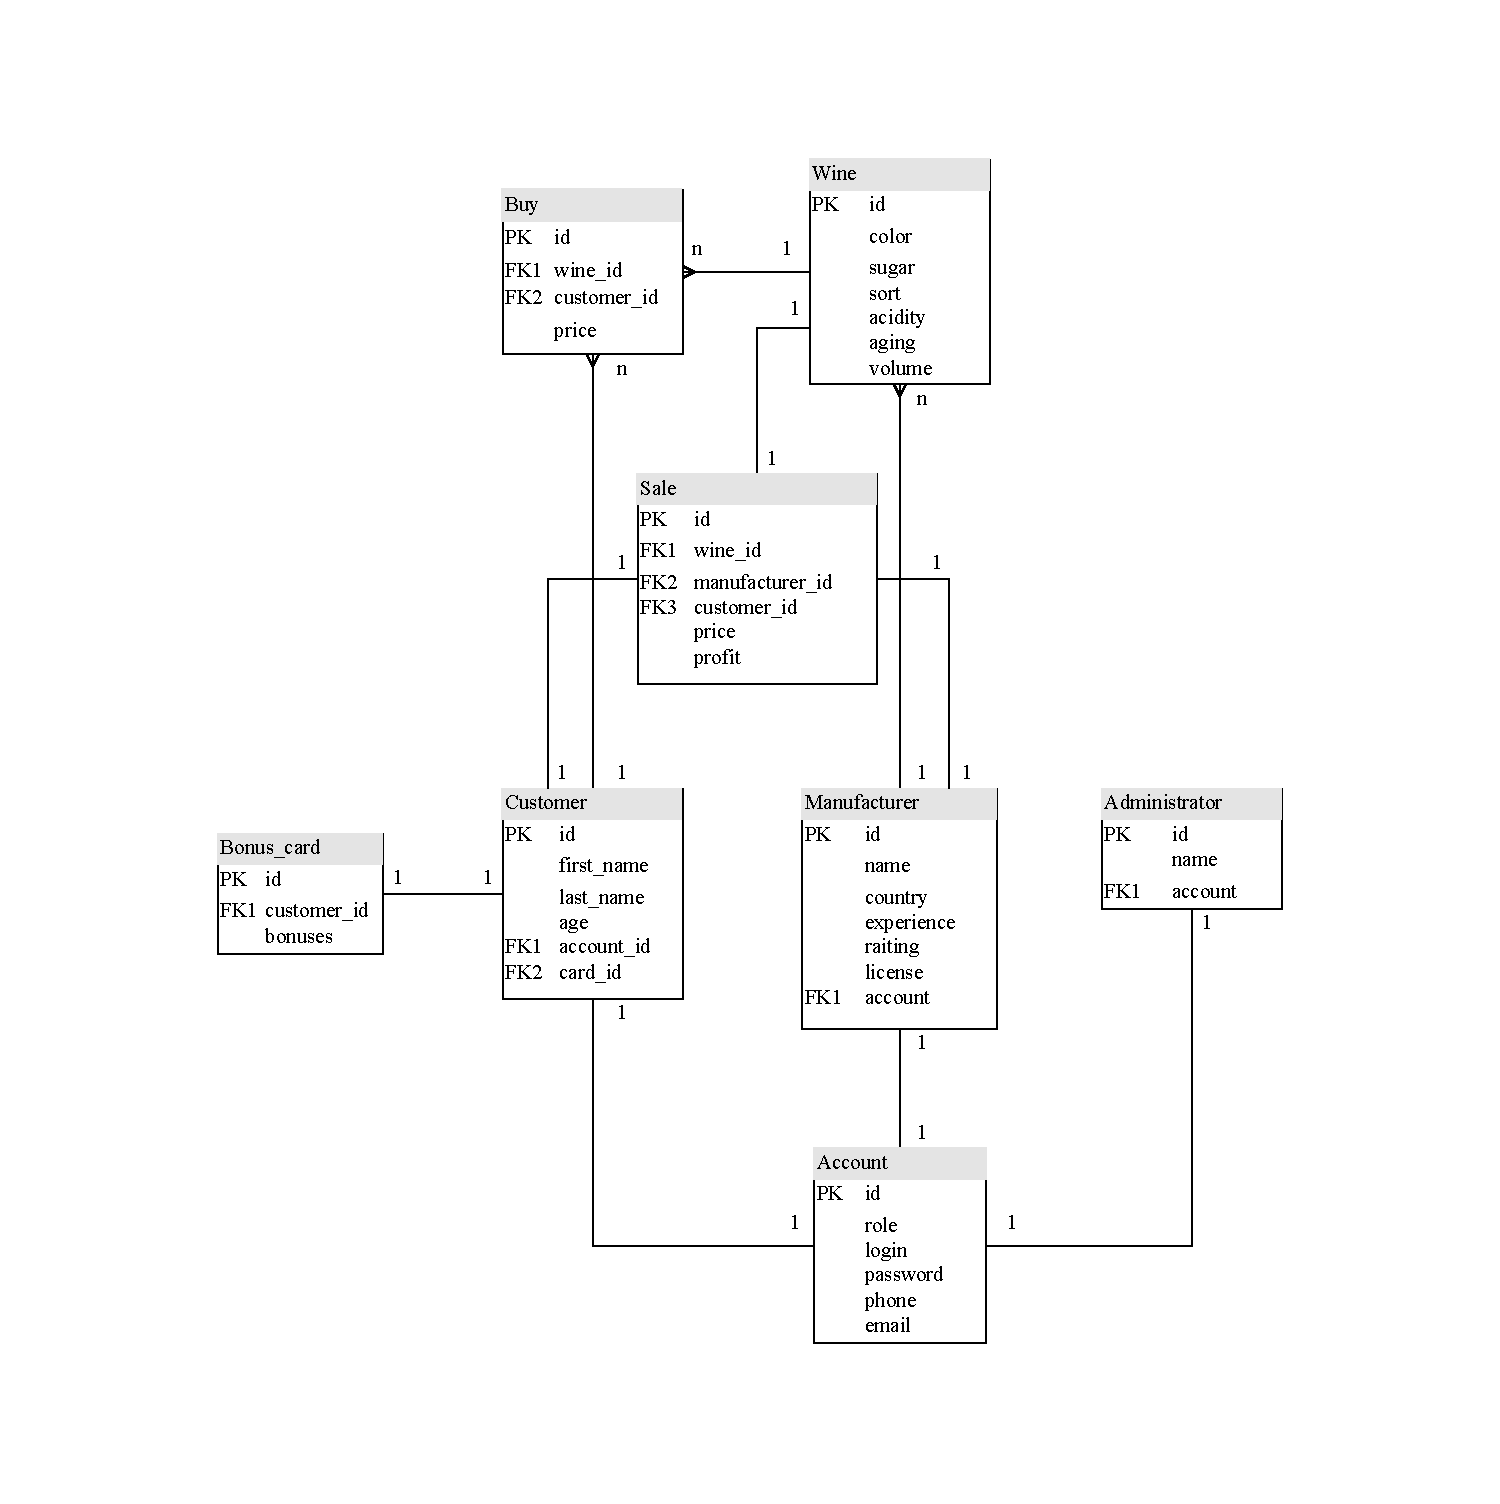
\includegraphics[scale=0.75]{img/ER-diagram.pdf}
	\end{center}
	\captionsetup{justification=centering}
	\caption{ER-диаграмма сущностей}
	\label{img:er}
\end{figure}

\section{Use-case диаграммы}

\begin{figure}[H]
	\begin{center}
		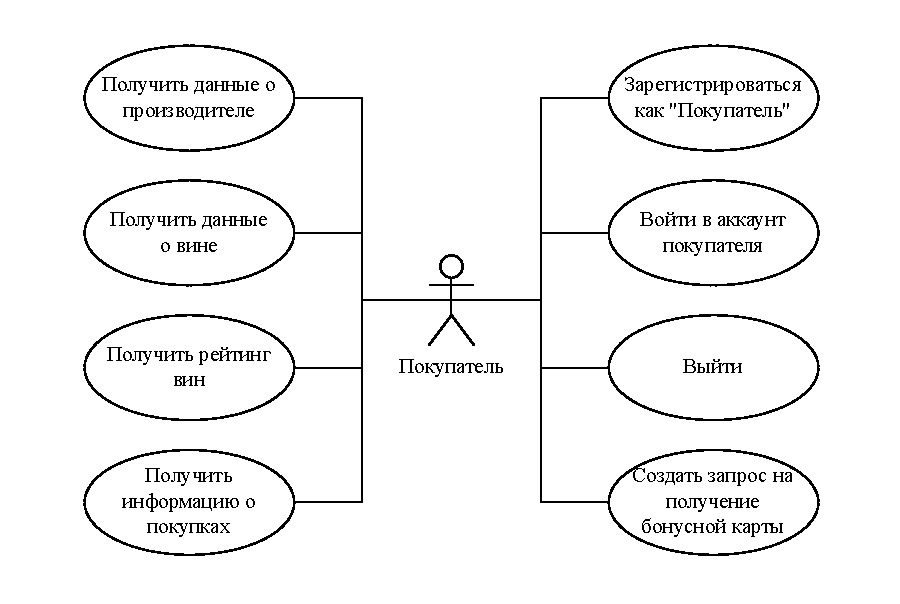
\includegraphics[scale=0.8]{img/customer.pdf}
	\end{center}
	\captionsetup{justification=centering}
	\caption{Use-case - покупатель}
	\label{img:customer}
\end{figure}

\begin{figure}[H]
	\begin{center}
		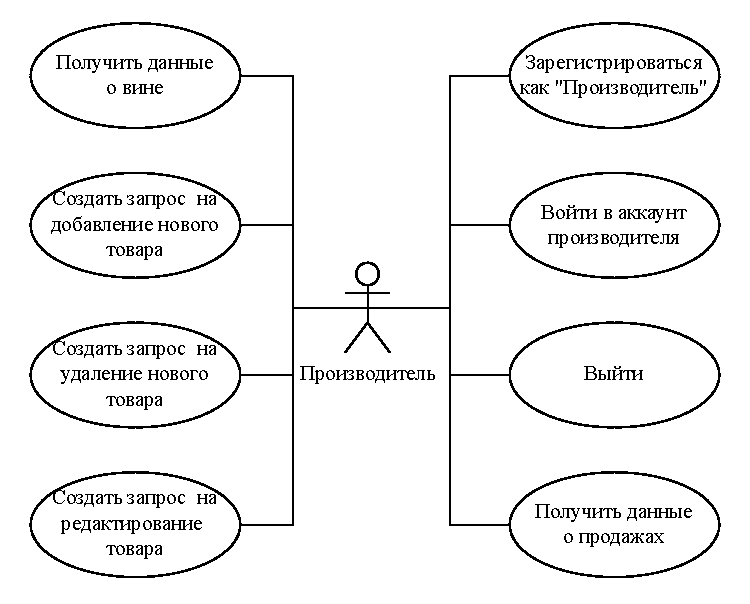
\includegraphics[scale=0.8]{img/manufacturer.pdf}
	\end{center}
	\captionsetup{justification=centering}
	\caption{Use-case - производитель}
	\label{img:manufacturer}
\end{figure}

\begin{figure}[H]
	\begin{center}
		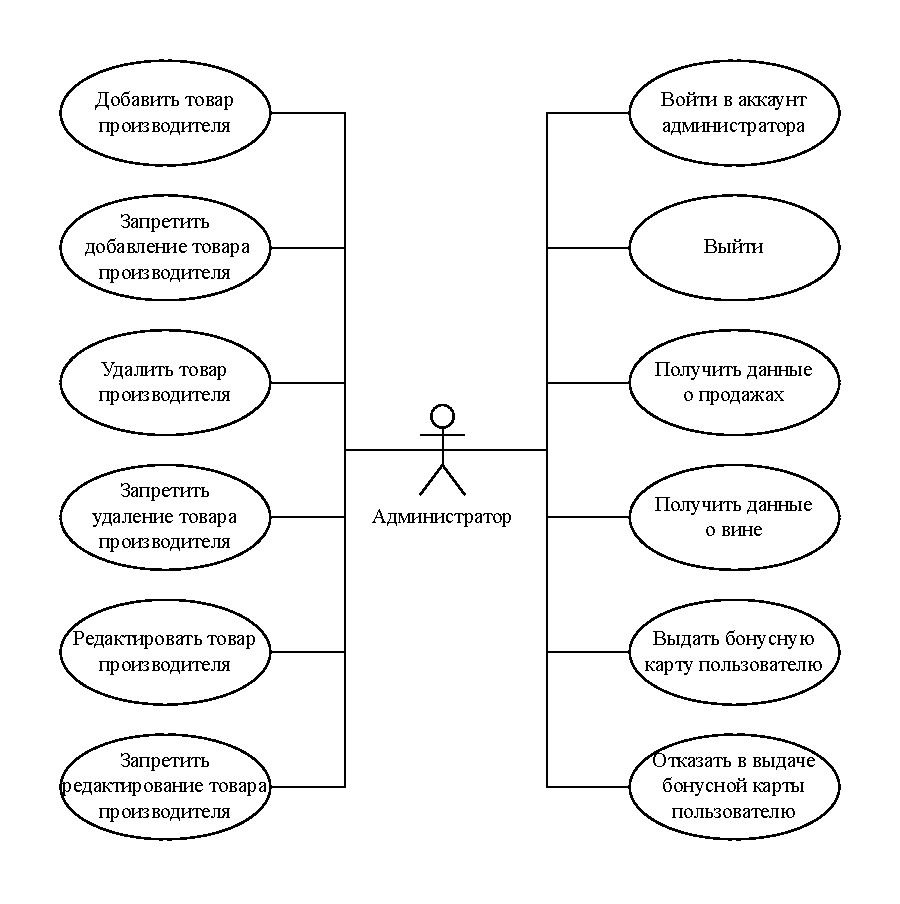
\includegraphics[scale=0.8]{img/administrator.pdf}
	\end{center}
	\captionsetup{justification=centering}
	\caption{Use-case - администратор}
	\label{img:administrator}
\end{figure}